%%%%%%%%%%%%%%%%%%%%%%%%%%%%%%%%%%%%%%%%%%%%%%%%%%%%%%%%%%
\frame {\frametitle{Spark Components}
%%%%%%%%%%%%%%%%%%%%%%%%%%%%%%%%%%%%%%%%%%%%%%%%%%%%%%%%%%
\begin{figure}[h]
  \centering
  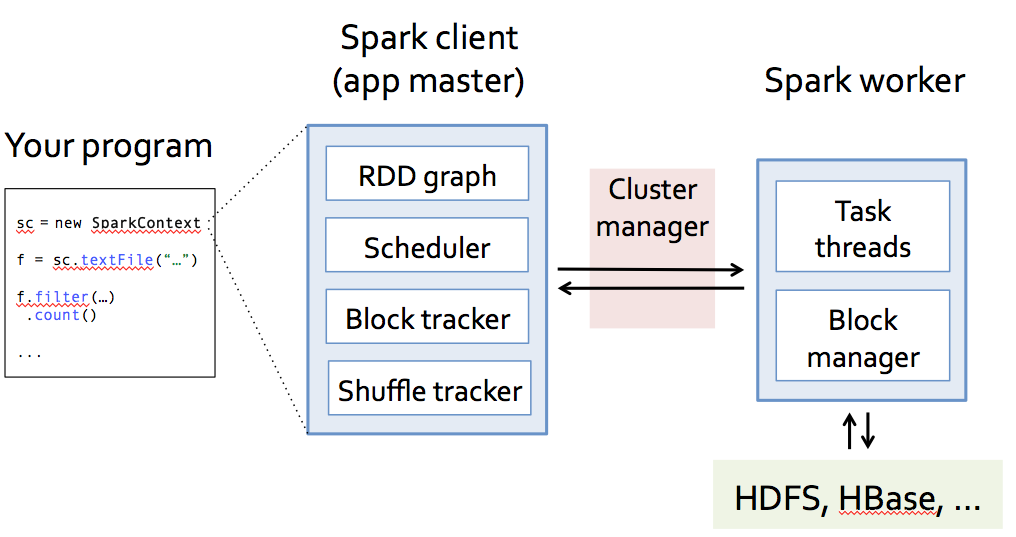
\includegraphics[scale=0.33]{./Figures/spark_components}
  \label{fig:spark_components}
\end{figure}
}

%%%%%%%%%%%%%%%%%%%%%%%%%%%%%%%%%%%%%%%%%%%%%%%%%%%%%%%%%%
% \frame {\frametitle{A Simple Job Example in Spark}
\begin{frame}[fragile]
\frametitle{A Simple Job Example in Spark}
%%%%%%%%%%%%%%%%%%%%%%%%%%%%%%%%%%%%%%%%%%%%%%%%%%%%%%%%%%


\begin{lstlisting}
val sc = new SparkContext("spark://...", "MyJob", home, jars) 

val file = sc.textFile("hdfs://...") // This is an RDD

val errors = file.filter(_.contains("ERROR")) // This is an RDD

errors.cache()

errors.count() // This is an action
\end{lstlisting}

\end{frame}

